%%%%%%%%%%%%%%%%%%%%%%%%%%%%%%%%%%%%%%%%%
% University/School Laboratory Report
% LaTeX Template
% Version 3.1 (25/3/14)
%
% This template has been downloaded from:
% http://www.LaTeXTemplates.com
%
% Original author:
% Linux and Unix Users Group at Virginia Tech Wiki 
% (https://vtluug.org/wiki/Example_LaTeX_chem_lab_report)
%
% License:
% CC BY-NC-SA 3.0 (http://creativecommons.org/licenses/by-nc-sa/3.0/)
%
% Modified by:
% Bartlomiej Dybisz
% Warsaw university of Technology
%
%%%%%%%%%%%%%%%%%%%%%%%%%%%%%%%%%%%%%%%%%

%----------------------------------------------------------------------------------------
%	PACKAGES AND DOCUMENT CONFIGURATIONS
%----------------------------------------------------------------------------------------

\documentclass{article}

\usepackage[version=3]{mhchem} % Package for chemical equation typesetting
\usepackage{siunitx} % Provides the \SI{}{} and \si{} command for typesetting SI units
\usepackage{graphicx} % Required for the inclusion of images
\usepackage{amsmath} % Required for some math elements 
\usepackage{url} % for bibliograpy links
\usepackage{float} % To force image to stand still
\usepackage[export]{adjustbox}
\usepackage[usenames, dvipsnames]{color} % to color some important remarks
\usepackage{caption}
\usepackage{wrapfig}
\usepackage{subcaption}
\urlstyle{same}  % (for bibliography links
\setlength\parindent{0pt} % Removes all indentation from paragraphs
%\usepackage{array}

\newenvironment{conditions}
  {\par\vspace{\abovedisplayskip}\noindent\begin{tabular}{>{$}l<{$} @{${}\equiv{}$} l}}
  {\end{tabular}\par\vspace{\belowdisplayskip}}
  
 \usepackage{amsfonts} 
\renewcommand{\labelenumi}{\alph{enumi}.} % Make numbering in the enumerate environment by letter rather than number (e.g. section 6)

%\usepackage{times} % Uncomment to use the Times New Roman font

%----------------------------------------------------------------------------------------
%	DOCUMENT INFORMATION
%----------------------------------------------------------------------------------------

\title{Analysis and Processing of Biometric Images \\ Laboratory 3} % Title

\author{Bartłomiej \textsc{Dybisz}} % Author name

\date{\today} % Date for the report

\begin{document}

\maketitle % Insert the title, author and date

\begin{center}
\begin{tabular}{l r}
Date Performed: & October 31 , 2015 \\ % Date the experiment was performed
Instructor: & mgr Piotr Panasiuk % Instructor/supervisor
\end{tabular}
\end{center}

% If you wish to include an abstract, uncomment the lines below
% \begin{abstract}
% Abstract text
% \end{abstract}

%----------------------------------------------------------------------------------------
%	SECTION 1
%----------------------------------------------------------------------------------------

\section{Objectives}

% If you have more than one objective, uncomment the below:
\begin{description}
\item[Convolution Filters] \hfill \\
To learn mathematics behind convolution filters in order to gain some intuition about them.
\item[High Pass Filter] \hfill \\
To learn how High Pass Filter works and how to implement it using Java.
\item[Low Pass Filter] \hfill \\
To learn how Low Pass Filter works and how to implement it using Java.
\item[Gaussian Filter] \hfill \\
To learn how Gaussian Filter works and how to implement it using Java. 
\item[Sobel Filter] \hfill \\
To learn how Sobel Filter works and how to implement it using Java.
\item[Erosion and Dilation] \hfill \\
To learn how Erosion and Dilation works. Although they were not implemented during laboratories, I will present straight forward implementation using Java. 
\item[Region Filling (Conditional Dilation)] \hfill \\
To learn how Conditional Dilation algorithm works. Region filling is another problem, which has been just mentioned during laboratories. I have decided to expand this report by introducing one of possible algorithm and its implementation in Java.
\item[Region Extraction] \hfill \\
To propose a way to extract a pupil, along with its diameter/radius and center, from an default input image.
This part has been left as a homework. It involves custom solution of the problem.
\end{description}

\subsection{Definitions}
\label{definitions}
\textcolor{red}{Remark:} throughout this report I will assume that each of red, green, blue channels of a pixel can take values from $0$ to $1$. It is imposed by JavaFX 8 - technology used to implement algorithms.

\begin{description}

%
% CONVOLUTION DEFINITION
%
\item[Convolution]
A convolution is an integral that expresses the amount of overlap of one function g as it is shifted over another function f. It therefore "blends" one function with another  \cite{convolution_wolphram}. 

In other words, convolution gives the area overlap between the two functions as a function of the amount that one of the original functions is translated \cite{convolution_wiki}.

Formally, for functions $f(x)$ and $g(x)$ of a continuous variable x, convolution is defined as:
\begin{equation} \label{conv_one_var_cont}
f(x) * g(x) = \int_{-\infty}^{\infty} f(\tau) \cdot g(x - \tau) d\tau
\end{equation}
, where $*$ means convolution operation, $\cdot$ represents common multiplication and $\tau$ is a "shifting variable".

Equation \ref{conv_one_var_cont} can be easily transformed to discrete form as follows:
\begin{equation} \label{conv_one_var_disc}
f[x] * g[x] = \sum_{k=-\infty}^{\infty} f[k] \cdot g[x-k]
\end{equation}
This form will be of particular interest for us, since it can be (more or less) directly applied to an image as showed in the next subsection.

%
% Convolution Filters
%
\item[Convolution Filters]
As mentioned, one can ad hoc transform equation \ref{conv_one_var_disc} into two variable case:
\begin{equation} \label{two_var_conv_one_var_disc}
f[x,y] * g[x,y] =\sum_{n_{1}=-\infty}^{\infty} \sum_{n_{2}=-\infty}^{\infty} f[n_{1}, n_{2}] \cdot g[x-n_{1}, y - n_{2}]
\end{equation}
, but for our purposes (as explained in a moment) we will use a slightly modified version of equation \ref{two_var_conv_one_var_disc}, namely:
\begin{equation} \label{final_two_var_conv_one_var_disc}
f[x,y] * g[x,y] = d \cdot (\sum_{n_{1}=k_{1}}^{k_{2}} \sum_{n_{2}=k_{3}}^{k_{4}} f[n_{1}, n_{2}] \cdot g[x+n_{1}, y + n_{2}])
\end{equation}
,where:
\begin{conditions} 
  d \in \mathbb{R} & scaling variable\\
  n_{1}, n_{2} \in \mathbb{N}& auxiliary shifting variables\\
  k_{1}, k_{2}, k_{3}, k_{4} \in \mathbb{N}& size restriction to convolution matrix (kernel)\\
 (x,y) \in \mathbb{N}^{2}     &  pixel of interest's position on an image in XY coordinates \\   
 f[x,y] : \mathbb{N}^{2} \rightarrow \mathbb{N} &  convolution matrix (kernel) \\
 g[x,y] : \mathbb{N}^{2} \rightarrow \mathbb{N} & an image as a matrix of pixels values
\end{conditions}

Equation \ref{two_var_conv_one_var_disc} has been changed due to obsolete $g[x-k]$ notation of equation \ref{conv_one_var_disc}. In this way we can omit left-right flipping when calculating consecutive pixels.

In addition, we restrict $g[x,y]$ by $k$'s variables, because we want our convolution matrix to be finite. 
In this case we can think of $f[x,y]$ as a frame, which we move over some pixel $(x,y)$ of an image $g[x,y]$. Then by applying equation \ref{final_two_var_conv_one_var_disc} we sum all values of $g$ over
$ \langle x + k_1; x+ k_2 \rangle \cup \langle y + k_3 ; y + k_4 \rangle$ interval multiplied by appropriate values of $f$.

What is more variable $d$ is a constant useful in computer implementation. I presume, that its main aim is to force kernel matrix values to stay in form of natural numbers.

As an example let us assume that:
\begin{conditions} 
  g[x,y] : \langle 1; 5 \rangle \cup \langle 1 ; 7 \rangle \rightarrow \mathbb{N} & some very small image\\
  f[x,y] : \langle -1; 1 \rangle \cup \langle -1 ; 1 \rangle \rightarrow \mathbb{N} & kernel matrix \\
\end{conditions}

In such a case we can present both of them in form of matrices of some natural values. Let us assume that figure \ref{fig:example_repr} defines $f[x,y]$ and $g[x,y]$ in terms of matrices. Value of $d$ will be 1.
\begin{figure}[H]
\centering
\begin{subfigure}{.4\textwidth}
  \centering
  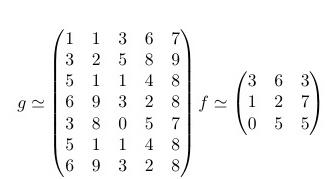
\includegraphics[width=0.95\linewidth]{_Figures/example_11.jpg}
  \caption{}
  \label{fig:example_repr}
\end{subfigure}%
\begin{subfigure}{.4\textwidth}
  \centering
  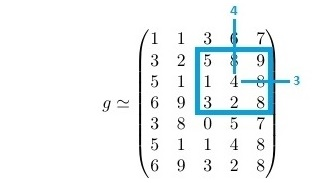
\includegraphics[width=0.95\linewidth]{_Figures/example_12.jpg}
  \caption{}
  \label{fig:example_43}
\end{subfigure}%
\caption{}
\label{fig:results_tresh}
\end{figure}

Now we want to apply convolution for let us say pixel $(4,3)$. Figure \ref{fig:example_43} represents region of interest. Equation \ref{final_two_var_conv_one_var_disc} for this case takes following form:
\begin{equation} 
\begin{split}
f[4,3] * g[4,3] =\sum_{n_{1}=-1}^{1} \sum_{n_{2}=-1}^{1} f[n_{1}, n_{2}] \cdot g[4+n_{1}, 3 + n_{2}] \\
= f[-1, -1] \cdot g[3, 2] + f[-1, 0] \cdot g[3, 3] + f[-1, 1] \cdot g[3, 4] \\
+ f[0, -1] \cdot g[3, 2] + f[0, 0] \cdot g[3, 3] + f[0, 1] \cdot g[0, 4] \\
+ f[1, -1] \cdot g[3, 2] + f[1, 0] \cdot g[3, 3] + f[1, 1] \cdot g[0, 4] \\
= 3 * 5 + 1 * 1 + 0 * 3 \\
+ 6 * 8 + 2 * 4 + 5 * 2 \\
+ 3 * 9 + 7 * 8 + 8 * 5 \\
= 205
\end{split}
\end{equation}

In this way pixel of output image, positioned at $(4,3)$ will have value $205$. When we apply convolution to all pixels in $g$ we will get an output (filtered) image.

\begin{figure}
\noindent
\begin{minipage}{0.3\textwidth}% adapt widths of minipages to your needs
	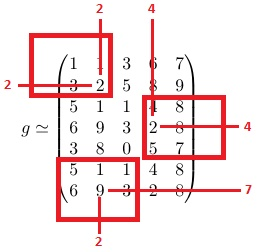
\includegraphics[width=\linewidth]{_Figures/conv_filter_border.jpg} 
	\caption{}
	\label{fig:caution}
\end{minipage}%
\hfill%
\begin{minipage}{0.6\textwidth}\raggedleft
\textcolor{red}{Caution:} Border cases i.e. cases when there is no corresponding $g[x,y]$ value for some value of $f[x,y]$ (see figure \ref{fig:caution} for reference), will be treated as special ones. In such a case pixel of interest will keep its value from $g$ function.
\end{minipage}
\end{figure}

\textcolor{red}{Remark:} If not stated otherwise, for the rest of the paper we will use only $3 \times 3$ kernel matrices, hence $k_1 = k_3 = -1$ and $k_2 = k_4 = 1$.

%
% HIG PASS FILTER DEFINITION
%
\item[High Pass Filter]
A high pass filter tends to retain the high frequency information within an image while reducing the low frequency information. The kernel of the high pass filter is designed to increase the brightness of the center pixel relative to neighbouring pixels. The kernel array usually contains a single positive value at its center, which is completely surrounded by negative values \cite{high_pass_def}. 

During laboratories we used following kernel:
\[
\begin{pmatrix}
  -1 & -1 & -1 \\
  -1 & 9 & -1 \\
  -1 & -1 & -1  \\
 \end{pmatrix}
 \]
with coefficient $d = \frac{1}{9}$ (see equation \ref{final_two_var_conv_one_var_disc} and previous subsection for a reference). 

%
% LOW PASS FILTER DEFINITION
%
\item[Low Pass Filter]
A low pass filter is the basis for most smoothing methods. An image is smoothed by decreasing the disparity between pixel values by averaging nearby pixels. Using a low pass filter tends to retain the low frequency information within an image while reducing the high frequency information \cite{high_pass_def}.

During laboratories we used following kernel:
\[
\begin{pmatrix}
  1 & 1 & 1 \\
  1 & 1 & 1 \\
  1 & 1 & 1  \\
 \end{pmatrix}
 \]
with coefficient $d = \frac{1}{9}$ (see equation \ref{final_two_var_conv_one_var_disc} and "Convolution Filters" subsection for a reference). 

%
% GAUSSIAN FILTER DEFINITION
% 
\item[Gaussian Filter] Type of image-blurring filter that uses a Gaussian function (which also expresses the normal distribution in statistics) for calculating the transformation to apply to each pixel in the image \cite{gaussian_blur}.

\begin{figure}[H]
\hskip 2.5em
\begin{minipage}{0.6\textwidth}\raggedright
The original pixel's value receives the heaviest weight (having the highest Gaussian value) and neighbouring pixels receive smaller weights as their distance to the original pixel increases. This results in a blur that preserves boundaries and edges better than other, more uniform blurring filters \cite{gaussian_blur}.
\end{minipage}
\begin{minipage}{0.3\textwidth}% adapt widths of minipages to your needs
	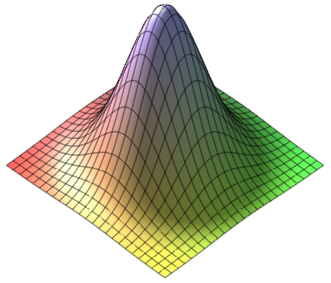
\includegraphics[width=\linewidth]{_Figures/gaussian.png} 
	\label{fig:caution}
\end{minipage}%
\hfill%
\end{figure}

During laboratories we used following kernel:
\[
\begin{pmatrix}
  1 & 4 & 1 \\
  4 & 16 & 4 \\
  1 & 4 & 1  \\
 \end{pmatrix}
 \]
with coefficient $d = \frac{1}{36}$ (see equation \ref{final_two_var_conv_one_var_disc} and "Convolution Filters" subsection for a reference). 

\item[Sobel Filter]
Performs a 2D spatial gradient measurement on an image and so emphasizes regions of high spatial frequency that correspond to edges \cite{sobel_bib1}.

Let us define $3 \times 3$ neighbourhood of pixel of interest $px$ as :
\[
N = 
\begin{pmatrix}
  p0 & p1 & p2 \\
  p7 & px & p3 \\
  p6 & p5 & p4
\end{pmatrix}
\]

To approximate appropriate derivatives on x ($G_x$) and y ($G_y$), we use following formulas:
\[
G_x =
\begin{pmatrix}
  -1 & -2 & -1 \\
   0 & 0 & 0 \\
   1 & 2 & 1
\end{pmatrix}
\times
N
\hskip 2.5em
G_y =
\begin{pmatrix}
  -1 & 0 & 1 \\
   -2 & 0 & 2 \\
   -1 & 0 & 1
\end{pmatrix}
\times
N
\]
, where $\times$ is an operation of matrix multiplication. What follows, values of each gradient can be directly calculated from neighbourhood pixels using following equations:
\[
\begin{split}
G_x = (p2 + 2 \cdot p3 + p4) - (p0 + 2 \cdot p7 + p6) \\
G_y = (p6 + 2 \cdot p5 + p4) - (p0 + 2 \cdot p1 + p2)
\end{split}
\]
Now output pixel value ($px_{out}$), based on gradient, can be calculated as:
\[
px_{out} = \sqrt{G_x^2 + G_y^2}
\]

\pagebreak

\item[Blur Filter]
Due to the demands of the task of pupil extraction, I needed some tool to blur an image to a higher degree than $3 \times 3$ Low Pass Filter or $3 \times 3$ Gaussian filter can. What is more, I could not allowed myself to not process border pixels. Because of all of this requirements simple extension to Low Pass Filter has been made.

Kernel is as follows:
\[
\begin{pmatrix}
  1 & 1 & 1 & 1 & 1 & 1 &1 \\
  1 & 1 & 1 & 1 & 1 & 1 &1 \\
  1 & 1 & 1 & 1 & 1 & 1 &1 \\
  1 & 1 & 1 & 1 & 1 & 1 &1 \\
  1 & 1 & 1 & 1 & 1 & 1 &1 \\
  1 & 1 & 1 & 1 & 1 & 1 &1 \\
  1 & 1 & 1 & 1 & 1 & 1 &1 
 \end{pmatrix}
 \]
with coefficient $d = \frac{1}{49 - \sigma}$, where $\sigma$ is number of pixels that can not be processed due to border case. In other words, for pixel of interest $px$, $\sigma$ represents number of $f[x,y]$ values for, which there is no corresponding $g[x,y]$ value (see equation \ref{final_two_var_conv_one_var_disc} and "Convolution Filters" subsection for a reference). 

%
% MORPHOLOGICAL IMAGE PROCESSING DEFINITION
%
\item[Morphological Image Processing] Is a collection of non-linear operations related to the shape or morphology of features in an image. According to \cite{morph_wiki}, morphological operations rely only on the relative ordering of pixel values, not on their numerical values, and therefore are especially suited to the processing of binary images.

Morphological techniques probe an image with a small shape or template called a structuring element. The structuring element is positioned at all possible locations in the image and it is compared with the corresponding neighbourhood of pixels \cite{morphological}.

%
% STRUCTING ELEMENT DEFINITION
%
\item[Structing Element] As stated in \cite{morphological}, structing element is a small binary image, i.e. a small matrix of pixels, each with a value of $0$ or $1$:

\begin{itemize}
\item The matrix dimensions specify the size of the structuring element.
\item The pattern of ones and zeros specifies the shape of the structuring element.
\item An origin of the structuring element is usually one of its pixels, although generally the origin can be outside the structuring element
\end{itemize}

Figure \ref{fig:struct_exampl} depicts squared, diamond-shaped and cross-shaped elements, respectively.
\begin{figure}[H]
  \centering
  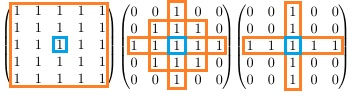
\includegraphics[width=0.7\linewidth]{_Figures/struct_el_example.jpg}
  \caption{Examples of structing element for morphological operations.}
  \label{fig:struct_exampl}
\end{figure}%


A common practice is to have odd dimensions of the structuring matrix and the origin defined as the centre of the matrix. Structuring elements play in morphological image processing the same role as convolution kernels in linear image filtering \cite{morphological}.

The structuring element is said to \textbf{fit} the image if, for each of its pixels set to 1, the corresponding image pixel is also 1. Similarly, a structuring element is said to \textbf{hit}, or intersect, an image if, at least for one of its pixels set to 1 the corresponding image pixel is also 1 \cite{morphological}.

\textcolor{red}{Remark:} In case of border pixels, I will follow pattern implemented in Matlab \cite{matlab}: during dilation, pixels beyond the image border are assigned the minimum value afforded by the data type (e.g in binary images, these pixels are assumed to be set to 0). On the other hand during erosion, such a pixels will take maximum value (again, for binary images binary images, these pixels are assumed to be set to 1).

%
% EROSION DEFINITION
%
\item[Erosion] We define erosion ($\ominus$) of binary image $f$ by structuring element $s$ as:
\[
    f \ominus s= (\forall{(x,y) \in f})  \;\;
    g(x,y) = 
\begin{cases}
    1,& \text{if s fits f }\\
    0,              & \text{otherwise}
\end{cases} 
\]
, where $g$ is output image and $g(x,y)$ denotes value of pixel of coordinate $(x,y)$ on $g$.

What is interesting erosion is equivalent to computing local minimum over the area of the structuring element. We scan the input image $f$, we compute minimal pixel value overlapped by $s$ and we replace pixel of interest with this value (we save it in $g$)\cite{slajdy_morph}.

Figure \ref{fig:erosion_exampl} presents erosion on small image with $3 \times 3$ squared-shaped structuring element.
\begin{figure}[H]
  \centering
  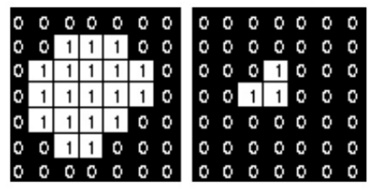
\includegraphics[width=0.4\linewidth]{_Figures/erosion_example.jpg}
  \caption{Example of erosion.}
  \label{fig:erosion_exampl}
\end{figure}%

%
% DILATION DEFINITION
%
\item[Dilation] We define dilation ($\oplus$) of binary image $f$ by structuring element $s$ as:
\[
    f \oplus s= (\forall{(x,y) \in f})  \;\;
    g(x,y) = 
\begin{cases}
    1,& \text{if s hits f }\\
    0,              & \text{otherwise}
\end{cases} 
\]
, where $g$ is output image and $g(x,y)$ denotes value of pixel of coordinate $(x,y)$ on $g$.

Dilation is converse of erosion. It gradually enlarges the boundaries of regions of foreground pixels. Thus areas of foreground regions grow in size, while holes within those regions become smaller \cite{slajdy_morph}.

Figure \ref{fig:dilation_exampl} presents dilation on small image with $3 \times 3$ squared-shaped structuring element.
\begin{figure}[H]
  \centering
  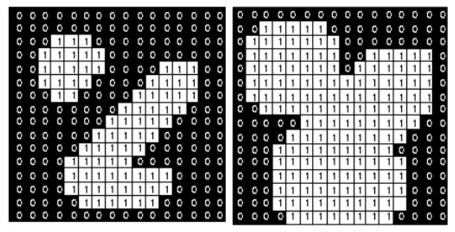
\includegraphics[width=0.4\linewidth]{_Figures/dilation_example.jpg}
  \caption{Example of dilation.}
  \label{fig:dilation_exampl}
\end{figure}%

%
% OPENING DEFINITION
% 
\item[Opening]
The opening of an image $f$  by a structuring element $s$ (denoted by $f \circ s$) is an erosion followed by a dilation \cite{morphological}: 
\[
f \circ s = (f \ominus s) \oplus s
\]
Opening is so called because it can open up a gap between objects connected by a thin bridge of pixels. Any regions that have survived the erosion are restored to their original size by the dilation.

In addition, opening is an idempotent operation: once an image has been opened, subsequent openings with the same structuring element have no further effect on that image \cite{morphological}:
\[
(f \circ s) \circ s = f \circ s
\]


%
% CLOSING DEFINITION
%
\item[Closing] The closing of an image $f$  by a structuring element $s$ (denoted by $f \bullet s$) is a dilation followed by an erosion: 
\[
f \bullet s = (f \oplus s_{rot}) \ominus s_{rot}
\]
, where $s_{rot}$ denotes structuring element rotated by $180^{o}$. In most cases $s$ will be symmetrical though.

Closing is so called because it can fill holes in the regions while keeping the initial region sizes. Like opening, closing is idempotent \cite{morphological}:
\[
(f \bullet s) \bullet s = f \bullet s
\]
%
% REGION FILLING ALGORITHM DEFINITION
%
\item[Region Filling (Conditional Dilation)]

\end{description} 
\pagebreak
 
%----------------------------------------------------------------------------------------
%	SECTION 2
%----------------------------------------------------------------------------------------

\section{Experimental Data}
During laboratory we used only one image (i.e. \ref{fig:sample_1}), but to enrich this report I will use another four of them. Since final task was to find pupil, I decided that all data will present human eyes.

\begin{figure}[H]
\centering
\begin{subfigure}{.5\textwidth}
  \centering
  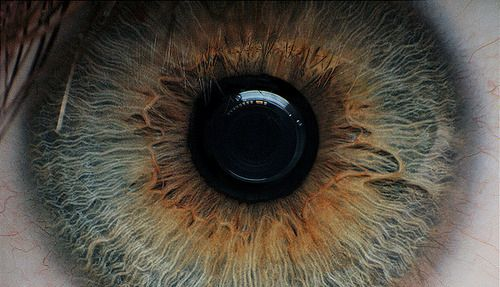
\includegraphics[width=0.97\linewidth]{_Figures/raw_data_1.jpg}
  \caption{}
  \label{fig:sample_1}
\end{subfigure}%
\begin{subfigure}{.5\textwidth}
  \centering
  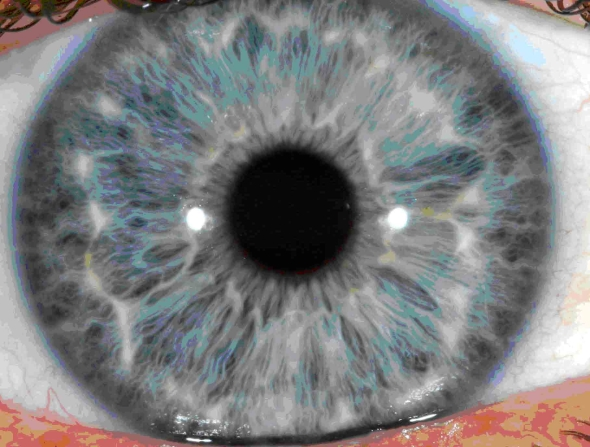
\includegraphics[width=0.97\linewidth]{_Figures/raw_data_2.jpg}
    \caption{}
  \label{fig:sample_2}
\end{subfigure}
\begin{subfigure}{.5\textwidth}
  \centering
  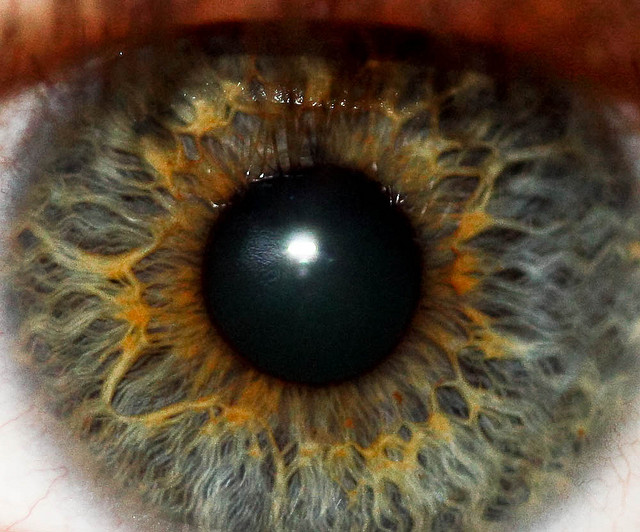
\includegraphics[width=0.97\linewidth]{_Figures/raw_data_3.jpg}
  \caption{}
  \label{fig:sample_3}
\end{subfigure}%
\begin{subfigure}{.5\textwidth}
  \centering
  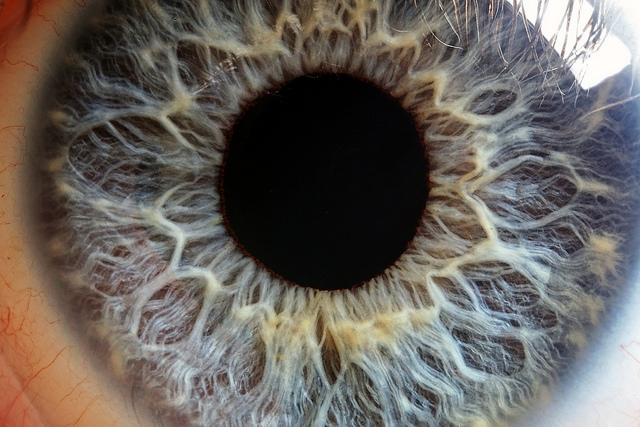
\includegraphics[width=0.97\linewidth]{_Figures/raw_data_4.jpg}
    \caption{}
  \label{fig:sample_4}
\end{subfigure}
\begin{subfigure}{.5\textwidth}
  \centering
  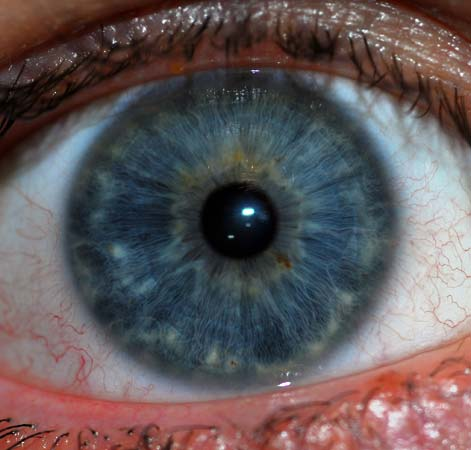
\includegraphics[width=0.6\linewidth]{_Figures/raw_data_5.jpg}
    \caption{}
  \label{fig:sample_4}
\end{subfigure}
\caption{Images used to check implemented algorithms.}
\label{fig:double_samples}
\end{figure}

\pagebreak

%----------------------------------------------------------------------------------------
%	SECTION 3
%----------------------------------------------------------------------------------------

\newpage
\section{Sample Code}
This section contains code snippets with algorithms implementation. Each figures is provided with appropriate description either in caption or in method's comment. 

%
% CLASS DIAGRAM
%
\subsection{Operations Class Diagram}


%
% CONVOLUTION FILTER CODE
%
\subsection{Convolution Filter Implementation}
\begin{figure}[H]
	\centering
	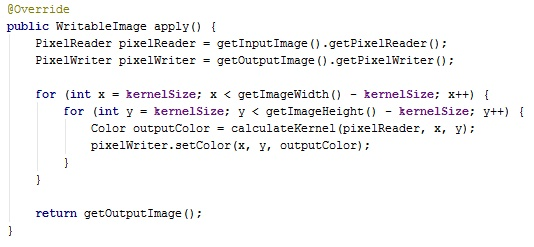
\includegraphics[width=0.97\textwidth]{_Figures/conv_filter_apply.jpg}
    \caption{Auxiliary method and fields value of HighPassFilter class.}
    \label{fig:code:treshold_func}
\end{figure}

\begin{figure}[H]
	\centering
	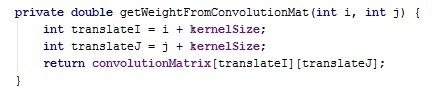
\includegraphics[width=0.8\textwidth]{_Figures/conv_filter_weight.jpg}
    \caption{Auxiliary method and fields value of HighPassFilter class.}
    \label{fig:code:treshold_func}
\end{figure}

\begin{figure}[H]
	\centering
	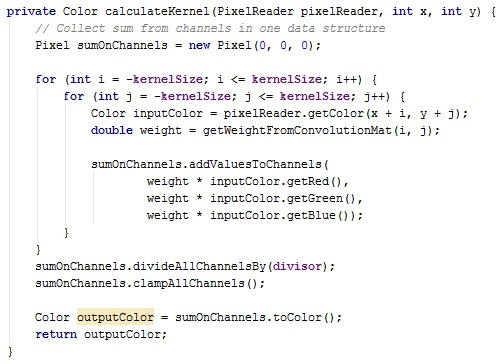
\includegraphics[width=0.97\textwidth]{_Figures/conv_filter_kernel.jpg}
    \caption{Auxiliary method and fields value of HighPassFilter class.}
    \label{fig:code:treshold_func}
\end{figure}


%
% HIGH PASS CODE
%
\subsection{High Pass Filter Implementation}
\begin{figure}[H]
	\centering
	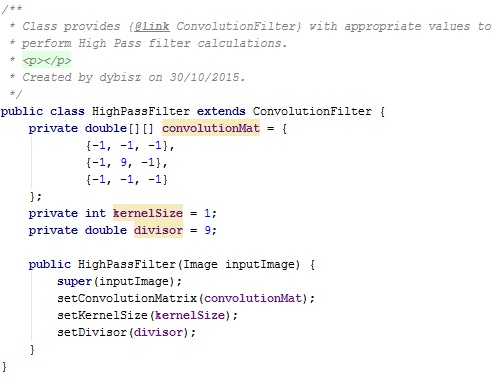
\includegraphics[width=0.97\textwidth]{_Figures/highpass_class.jpg}
    \caption{Auxiliary method and fields value of HighPassFilter class.}
    \label{fig:code:treshold_func}
\end{figure}

%
% LOW PASS CODE
%
\subsection{Low Pass Filter Implementation}
\begin{figure}[H]
	\centering
	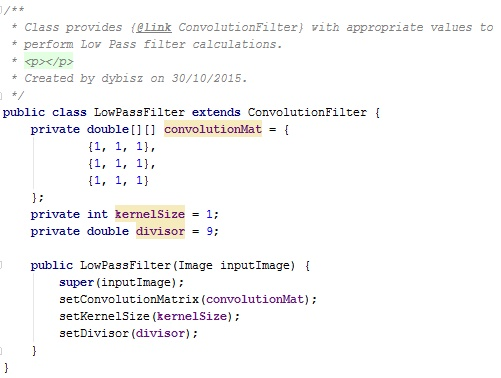
\includegraphics[width=0.97\textwidth]{_Figures/lowpass_class.jpg}
    \caption{Auxiliary method and fields value of HighPassFilter class.}
    \label{fig:code:treshold_func}
\end{figure}

%
% GAUSSIAN FILTER CODE
%
\subsection{Gaussian Filter Implementation}
\begin{figure}[H]
	\centering
	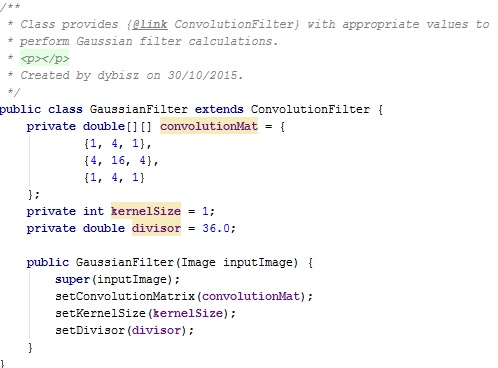
\includegraphics[width=0.97\textwidth]{_Figures/gaussian_class.jpg}
    \caption{Auxiliary method and fields value of HighPassFilter class.}
    \label{fig:code:treshold_func}
\end{figure}



%----------------------------------------------------------------------------------------
%	SECTION 4
%----------------------------------------------------------------------------------------

\section{Results and Conclusions}


%----------------------------------------------------------------------------------------
%	BIBLIOGRAPHY
%----------------------------------------------------------------------------------------
\newpage

\begin{thebibliography}{1}
	\bibitem{convolution_wolphram} \url{http://mathworld.wolfram.com/Convolution.html}
	\bibitem{convolution_wiki} \url{https://en.wikipedia.org/wiki/Convolution}
	\bibitem{convolution_equations} \url{https://graphics.stanford.edu/courses/cs178/applets/convolution.html}
	\bibitem{high_pass_def} \url{http://northstar-www.dartmouth.edu/doc/idl/html_6.2/Filtering_an_Imagehvr.html}
	\bibitem{gaussian_blur} \url{https://en.wikipedia.org/wiki/Gaussian_blur}
	\bibitem{sobel_bib1} \url{http://homepages.inf.ed.ac.uk/rbf/HIPR2/sobel.htm}
	\bibitem{morph_wiki} \url{https://en.wikipedia.org/wiki/Mathematical_morphology}	
	\bibitem{morphological} \url{https://www.cs.auckland.ac.nz/courses/compsci773s1c/lectures/ImageProcessing-html/topic4.htm}		
	\bibitem{matlab} \url{http://www.mathworks.com/help/images/morphology-fundamentals-dilation-and-erosion.html}
	\bibitem{slajdy_morph} \url{http://www.slideshare.net/vinayaknarayanan/morphological-image-processing-12323183}
	
\end{thebibliography}

%----------------------------------------------------------------------------------------


\end{document}